\TChapter{Avances}{epsilon}
\ \\\\
En esta sección se mostrarán los avances que hasta el día de hoy se tienen.

\section{Herramientas utilizadas}
Para el desarrollo de los avances en el presente trabajo, se utilizó el lenguaje de programación Python\footnote{https://www.python.org/}, 
que nos ofrece multiples librerías para el análisis de datos. Debido a que muchas librerias científicas requieren una versión específica 
de Python se utilizó Anaconda\footnote{https://www.anaconda.com/distribution/} el cual proporciona una gran colección de bibliotecas de 
ciencia de datos altamente optimizadas y de uso común. Mientras que para el web-crawling se utilizó Scrapy\footnote{https://scrapy.org/}, 
el cual es un framework que permite la extracción de información de sitios web.

\section{Estudio previo}
Una vez que se eligieron las herramientas que permiten la extracción de la información, se procedió con la selección de los 
sitios web de los cuales se extraerían noticias, que posteriormente serán de ayuda para el entrenamiento del clasificador.
\\
El sitio web El Economista\footnote{https://www.eleconomista.com.mx/} contiene una sección llamada \textbf{Ranking de Medios Nativos Digitales}, 
la cual permite mostar estadísticas que realiza mes con mes acerca de los sitios web más consultados desde diferentes dispositivos electrónicos 
(Móviles, tabletas y escritorio).
El análisis se realizó sobre los dispositivos de escritorio, ya que el sistema propuesto será una aplicación web; como se observa en la Figura
 \textbf{\ref{fig:rank}} se podrán observar los sitios web más consultados.
\begin{figure}[H]
  \centering
  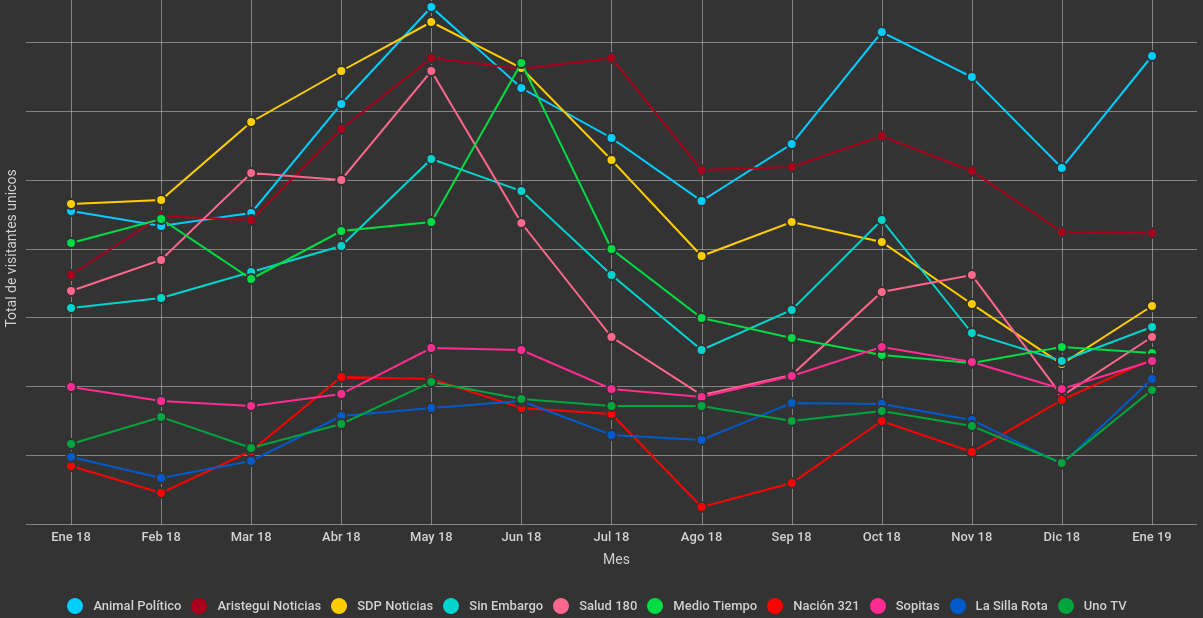
\includegraphics[scale=.28]{imagenes/Capitulo5/ranking}
  \caption{Ranking de sitios web del periodo de enero del 2018 a enero del 2019.}
  \label{fig:rank}
\end{figure}

Para el proceso de selección de los sitios web, se tomo en cuenta la publicación realizada, se eligieron 9 sitios web para su análisis:

\begin{itemize}
    \item 3 Sitios de foros de noticias: Aristegui Noticias, SDP Noticias y Sopitas.
    \item 3 Sitios de diarios: El Universal, La Jornada y Excelsior.
    \item 3 Sitios televisivos: TV Azteca, Televisa y Once Noticias.
\end{itemize}

Una vez seleccionados los sitios, se procedió con el análisis de las secciones que contiene cada sitio, como lo muestra el Cuadro \textbf{\ref{tabla:sitios}}.
\begin{table}[htbp]
    \centering
    \resizebox{\columnwidth}{!}{%
    \begin{tabular}[H]{|l|l|l|l|l|l|l|l|l|l|}
    \multicolumn{1}{l}{Sección}
    & \multicolumn{1}{l}{El Universal}
    & \multicolumn{1}{l}{La Jornada}
    & \multicolumn{1}{l}{Milenio} 
    & \multicolumn{1}{l}{Aristegui Noticias} 
    & \multicolumn{1}{l}{SDP Noticias} 
    & \multicolumn{1}{l}{Sopitas} 
    & \multicolumn{1}{l}{Azteca Noticias} 
    & \multicolumn{1}{l}{Televisa} 
    & \multicolumn{1}{l}{Once Noticias} \\ \cline{1-10}
        Nacional      & Nacional      & -            & Nacional      & México                & Nacional      & Noticias  & -                 & Nacional      & Nacional      \\ \hline
        Internacional & Mundo         & Mundo        & Mundo         & Destacado/Mundo       & Internacional & -         & Internacional     & Internacional & Internacional \\ \hline
        Ciudad        & Metrópoli     & Capital      & CDMX          & -                     & -             & -         & -                 & CDMX          & CDMX      \\ \hline
        Estados       & Estados       & Estados      & Estados       & Sociedad/México       & Estados       & -         & Estados           & Estados       & Nacional   \\ \hline
        Economía      & Cartera       & Economía     & Negocios      & Economía              & Economía      & -         & Finanzas          & Economía      & Economía   \\ \hline
        Deportes      & Deportes      & Deportes     & La Afición    & Deportes              & Deportes      & Deportes  & -                 & Deportes      & Deportes   \\ \hline
        Espectáculos  & Espectáculos  & Espectáculos & Hey           & -                     & En el show    & Entretenimiento & -           & Entretenimiento & Deportes    \\ \hline
        Cultura       & Cultura       & Cultura      & Cultura       & -                     & -             & -         & -                 & Arte y cultura & Cultura   \\ \hline
        Política      & Nación/política & Política   & Política      & Poderes               & -             & -         & Política          & Política      & -   \\ \hline
  Ciencia y tecnología& Ciencia y salud & Tecnología & Tecnología    &                       & Geek          & Geek      & -                 & Tecnología*      & Ciencia  \\ \hline        
    \end{tabular}%
}
\caption[Tabla]{Secciones existentes en los sitios web}
\label{tabla:sitios}
\end{table}
Una vez que se obtuvieron los resultados de las secciones, se definieron 5 secciones las cuales se consideran las más comunes dentro de los sitios web,

\begin{itemize}
    \item Política
    \item Deportes
    \item Ciencia y tecnología
    \item Economía
    \item Cultura
\end{itemize}


Para llevar a cabo el proceso de desarrollo del código que permite la extracción de la información, se realizó el estudio de la estructura XML
(Extensible Markup Language) de los sitios web seleccionados, con el fin de definir las etiquetas que contienen la información requerida.
Scrapy es una herramienta que permite la extracción de información de distintos sitios web, basado en las etiquetas de lo.
\\
De cada sitio web se analizó la estructura de la siguiente información contenida en cada noticia.\\
\begin{itemize}
  \item URL.
  \item Sección.
  \item Título.
  \item Autor.
  \item Fecha.
  \item Descripción.
  \item Noticia.
\end{itemize} 

\section{Recolección de noticias}
Para describir como se lleva a cabo la recolección de noticias se muestra en la siguiente Figura \textbf{\ref{fig:diagrama}}.

\begin{figure}[H]
  \centering
  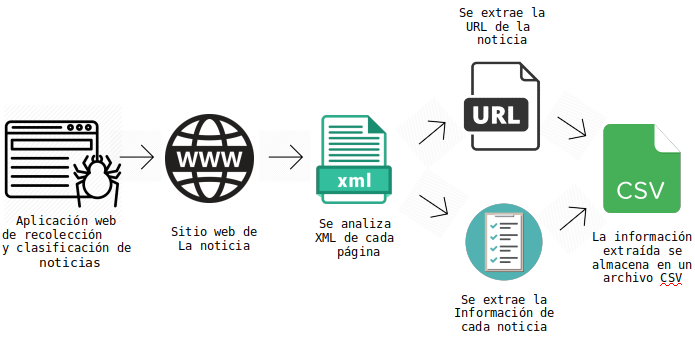
\includegraphics[scale=.50]{imagenes/Capitulo5/diagrama}
  \caption{Proceso de recolección de noticias.}
  \label{fig:diagrama}
\end{figure}

\subsection{Prerrequisitos}
\begin{itemize}
    \item Tener instalado en nuestro computador alguna distribución de Linux.
    \item Tener instalado python en a partir de su versión 2.7
    \item Tener conocimientos de la creación de entornos de desarrollo.
\end{itemize}

Para este proceso se abre una terminal nueva con la ruta donde se desee guardar el proyecto, Figura \textbf{\ref{fig:uno}} 

\begin{figure}[H]
  \centering
  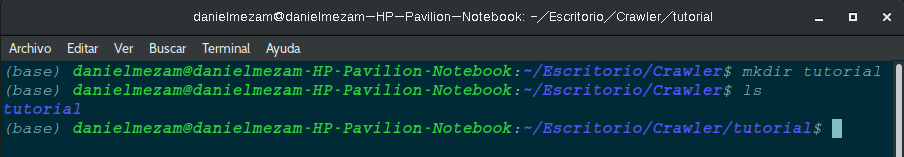
\includegraphics[scale=.35]{imagenes/Capitulo5/1}
  \caption{Carpeta donde se creará el proyecto.}
  \label{fig:uno}
\end{figure}

Una vez ubicados en la carpeta donde se creará el proyecto se procede con la creación de un entorno virtual y ahí se activará el entorno virtual 
creado Figura \textbf{\ref{fig:dos}}.

\begin{figure}[H]
    \centering
    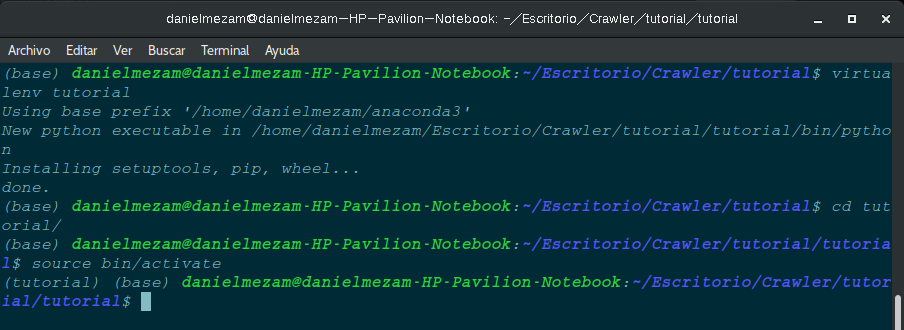
\includegraphics[scale=.35]{imagenes/Capitulo5/2}
    \caption{Creación del entorno virtual.}
    \label{fig:dos}
  \end{figure}

Una vez activado el entorno virtual, se procederá con la instalación de Scrapy y la creación del proyecto con la siguiente línea
\textbf{\textit{scrapy startproject tutorial}} Figura \textbf{\ref{fig:tres}} .

\begin{figure}[H]
    \centering
    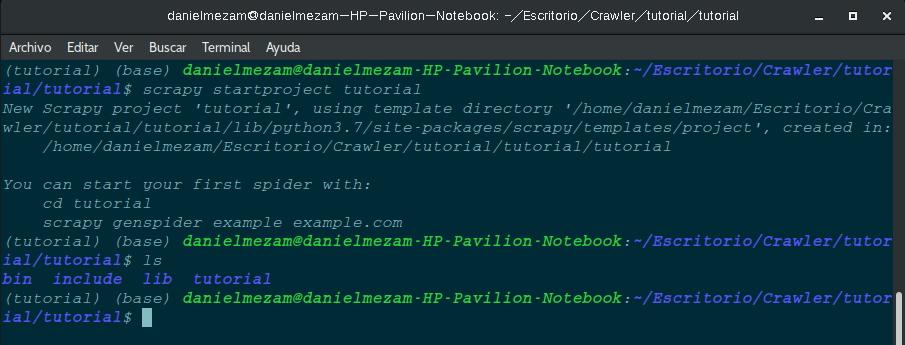
\includegraphics[scale=.35]{imagenes/Capitulo5/3}
    \caption{Creación del proyecto Scrapy.}
    \label{fig:tres}
  \end{figure}

Veremos que se ha creado una carpeta con el nombre del proyecto \textbf{"tutorial"}, la cual contiene los siguientes archivos Figura \textbf{\ref{fig:cuatro}} .

\begin{figure}[H]
    \centering
    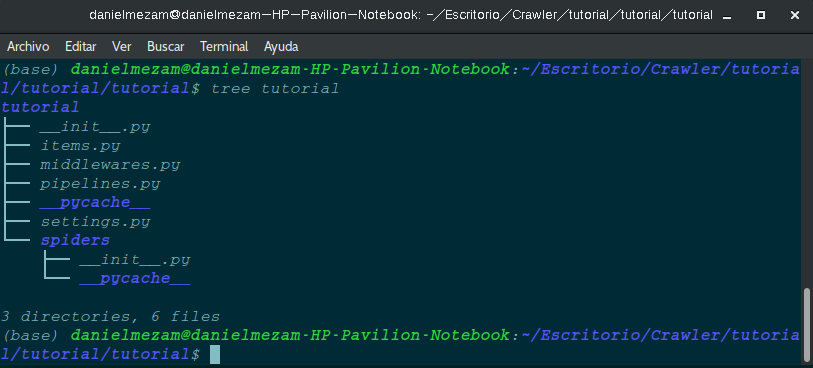
\includegraphics[scale=.35]{imagenes/Capitulo5/4}
    \caption{Carpetas y archivos creados.}
    \label{fig:cuatro}
  \end{figure}
 
Se definieron en el archivo \textbf{items.py} las etiquetas de la página que se necesita recolectar de cada noticia Figura \textbf{\ref{fig:cinco}}. 
\\
\begin{itemize}
  \item URL: Se necesita la URL para redireccionar al usuario a la página origen de la noticia seleccionada.
  \item Sección: Se necesita saber la sección para que sea de apoyo para el clasificador.
  \item Título: El título de la noticia permite al usuario saber sobre la noticia.
  \item Autor: Permite mostrar al usuario el autor de la noticia.
  \item Fecha: Se necesita la fecha para su clasificación por la fecha de publicación de la noticia.
  \item Descripción: Se mostrara al usuario una pequeña descripción de la noticia si es que la tiene.
  \item Noticia: El contenido de la noticia permite determinar la clasificación de la misma.
\end{itemize}
Es fundamental obtener toda la información de las etiquetas definidas la cual permitirá al clasificador obtener mejores resultados.
\\
Se procede con la creación un archivo dentro de la carpeta Spiders llamado \textbf{\textit{spiders.py}}, dentro de este archivo se encuentra el código 
de nuestras reglas XML para la extracción de la información.

\begin{figure}[H]
  \centering
  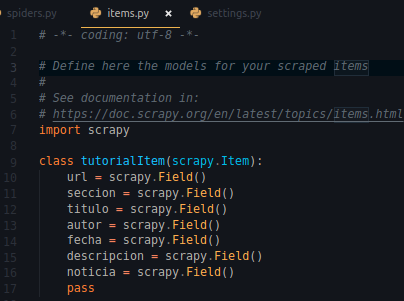
\includegraphics[scale=.45]{imagenes/Capitulo5/5}
  \caption{Información necesaria de extraer de cada noticia.}
  \label{fig:cinco}
\end{figure}

Se debe tener cuidado en la definición de las etiquetas XML, ya que de no ser bien definidas no se podrá extraer la información necesaria 
para el clasificador.
\\

\begin{figure}[H]
  \centering
  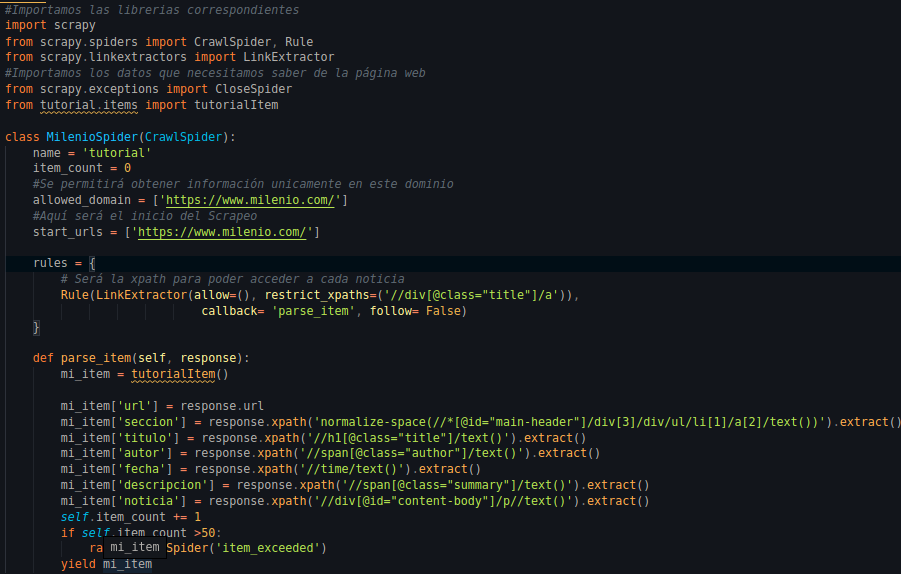
\includegraphics[scale=.45]{imagenes/Capitulo5/6}
  \caption{En la primera se muestran las librerias, posteriormente se definen las reglas las cuales son diferentes para cada sitio web.}
  \label{fig:seis}
\end{figure}

Una vez definidas las reglas que permiten la extracción, se procede a modificar el archivo \textbf{pipelines.py} el cual permite realizar 
la importación de la información obtenida a un archivo con formato CSV Figura \textbf{\ref{fig:siete}}
\\
\begin{figure}[H]
  \centering
  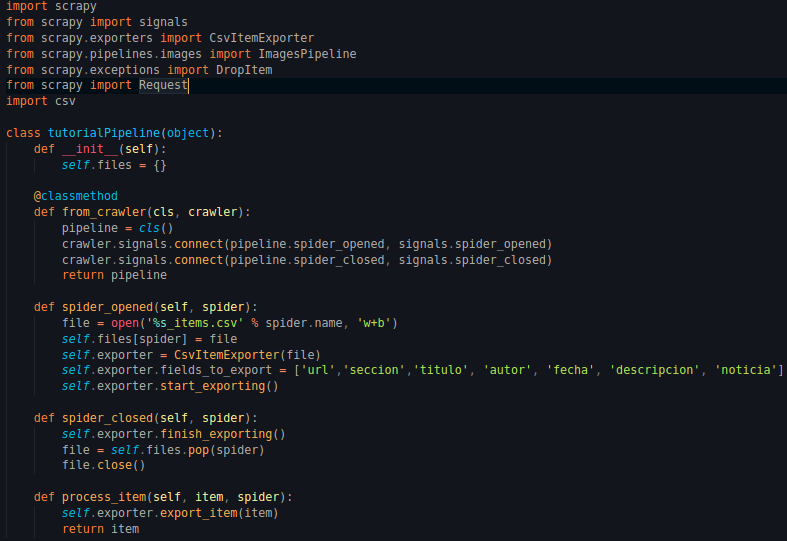
\includegraphics[scale=.45]{imagenes/Capitulo5/7}
  \caption{Código necesario para la exportación de la información extraída.}
  \label{fig:siete}
\end{figure}

Por último se procede con la ejecución del siguiente comando para extraer la información \textbf{scrapy crawl tutorial -t csv} Figura \textbf{\ref{fig:ocho}}

\begin{figure}[H]
  \centering
  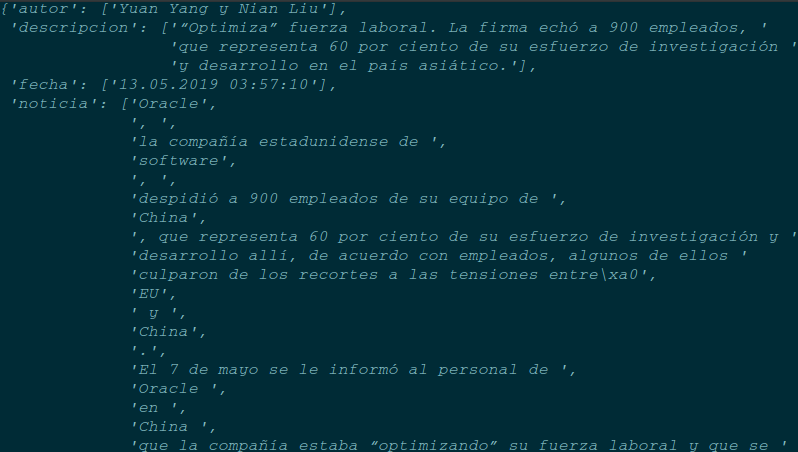
\includegraphics[scale=.35]{imagenes/Capitulo5/8}
  \caption{Muestra de la recolección realizada por el crawler.}
  \label{fig:ocho}
\end{figure}

\subsection{Resultados}
Una vez que termina de ejecutarse el crawler se genera un archivo CSV, ahí se almacena la información recolectada, posteriormente toda la información 
que se recolecto será utilizada para el algoritmo de entrenamiento Figura \textbf{\ref{fig:nueve}}.

\begin{figure}[H]
  \centering
  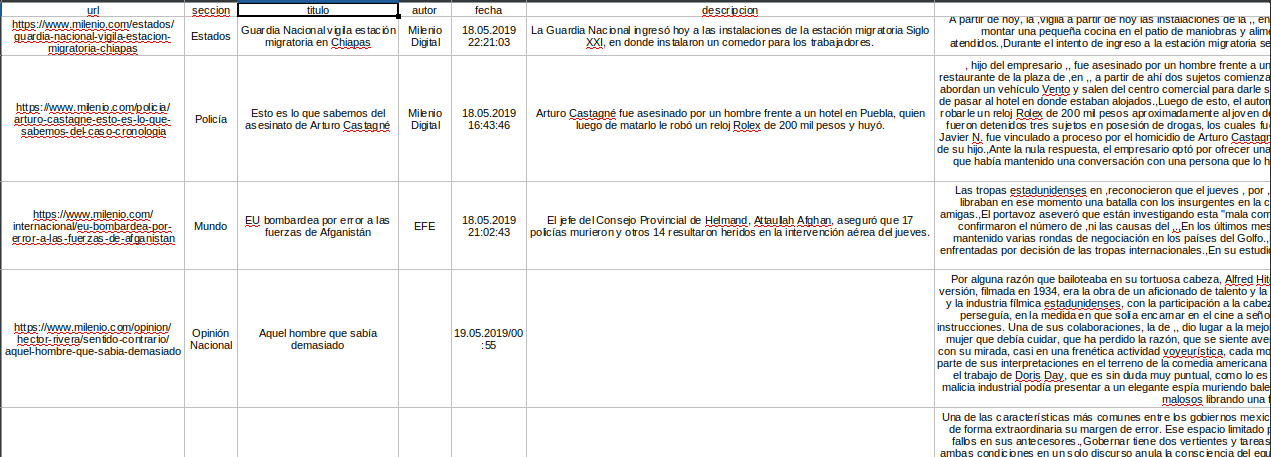
\includegraphics[scale=.30]{imagenes/Capitulo5/9}
  \caption{Resultados obtenidos de la extracción del sitio web almacenado en un archivo CSV.}
  \label{fig:nueve}
\end{figure}

\subsubsection{Resultados de las etiquetas}
De los nueve sitios elegidos para la recolección de noticias, se logró recolectar información de las etiquetas de cada sitio Tabla \textbf{\ref{tabla:etiquetas}}:
\\
\begin{table}[htbp]
  \centering
  \resizebox{\columnwidth}{!}{%
  \begin{tabular}{|l|l|l|l|l|l|l|l|l|l|}
  \multicolumn{1}{l}{Etiqueta}
  & \multicolumn{1}{l}{El Universal}
  & \multicolumn{1}{l}{La Jornada}
  & \multicolumn{1}{l}{Milenio} 
  & \multicolumn{1}{l}{Aristegui Noticias} 
  & \multicolumn{1}{l}{SDP Noticias} 
  & \multicolumn{1}{l}{Sopitas} 
  & \multicolumn{1}{l}{Azteca Noticias} 
  & \multicolumn{1}{l}{Televisa} 
  & \multicolumn{1}{l}{Once Noticias} \\ \cline{1-10}
      URL         & Sí & Sí & Sí & Sí & Sí & Sí & Sí & Sí & Sí \\ \hline
      Sección     & Sí & Sí & Sí & Sí & Sí & Sí & Sí & Sí & Sí \\ \hline
      Título      & Sí & Sí & Sí & Sí & Sí & Sí & Sí & Sí & Sí \\ \hline
      Autor       & Sí & Sí & Sí & Sí & Sí & Sí & Sí & Sí & Sí \\ \hline
      Fecha       & Sí & Sí & Sí & Sí & Sí & Sí & Sí & Sí & Sí \\ \hline
      Descripción & Sí & No & Sí & No & No & Sí & Sí & Sí & Sí \\ \hline
      Noticia     & Sí & Sí & Sí & Sí & Sí & Sí & Sí & Sí & Sí \\ \hline
    \end{tabular}%
\label{tabla:etiquetas}
}
\end{table}

A pesar de extraer la mayoría de etiquetas requeridas, existen algunos datos que se encuentran en una sola etiqueta.
\\
La mayor parte de los sitios permiten la extracción de noticias, sin embargo se debe tener cuidado que las etiquetas se 
encuentren bien descritas, de lo contrario no extrae información.
\subsubsection{Secciones recolectadas}

De los nueve sitios web definidos se obtuvieros las siguientes secciones Tabla \textbf{\ref{tabla:secciones}}:
\\
\begin{table}[htbp]
  \centering
  \resizebox{\columnwidth}{!}{%
  \begin{tabular}{|l|l|l|l|l|l|l|l|l|l|}
  \multicolumn{1}{l}{Sección}
  & \multicolumn{1}{l}{El Universal}
  & \multicolumn{1}{l}{La Jornada}
  & \multicolumn{1}{l}{Milenio} 
  & \multicolumn{1}{l}{Aristegui Noticias} 
  & \multicolumn{1}{l}{SDP Noticias} 
  & \multicolumn{1}{l}{Sopitas} 
  & \multicolumn{1}{l}{Azteca Noticias} 
  & \multicolumn{1}{l}{Televisa} 
  & \multicolumn{1}{l}{Once Noticias} \\ \cline{1-10}
      %                        1    2    3    4    5    6    7    8    9
      Economía              & Sí & Sí & Sí & Sí & Sí & No & Sí & Sí & Sí \\ \hline
      Deportes              & Sí & Sí & Sí & Sí & Sí & Sí & No & Sí & Sí \\ \hline
      Cultura               & Sí & Sí & Sí & No & No & No & No & Sí & Sí \\ \hline
      Política              & Sí & Sí & Sí & Sí & No & No & Sí & Sí & No \\ \hline
      Ciencia y tecnología  & Sí & Sí & Sí & No & Sí & Sí & No & Sí & Sí \\ \hline
    \end{tabular}%
\label{tabla:secciones}
}
\end{table}
\\
Cerca del 75\% de los sitios web seleccionados contienen las secciones que fueron definidas, 
debido a que los sitios web de foros de noticias (Aristegui Noticias, SDP Noticias y Sopitas) 
tienen muy pocas seccioned definidas dentro de su sitio web.
\subsection{Consideraciones}
\begin{itemize}
  \item Se debe tener conocimiento de XML para poder realizar las reglas que permitirán extraer información de la página web que se solicite extraer 
  información
  \item Cuando la noticia consta de un video, no se obtiene ninguna información adicional de la noticia.
  \item Se debe tomar en cuenta que las secciones no están homogeneizadas, es decir a pesar de que de la misma página existan varias secciones 
  \item La distribución de la información varia dependiendo a la sección y sitio web.
  \item Se acoto el periodo de busqueda de noticias ya que algunos sitios web muestran las noticias más recientes.
\end{itemize}

\section{Trabajo a futuro}
\begin{itemize}
  \item Una vez que se obtuvo la extracción de las noticias, se pretende que las noticias formaran parte del corpus.
  \item Corregir las reglas para la extracción de la información de los sitios web, y así evitar extraer información con código HTML.
  \item Agregar reglas para cada etiqueta, de manera tal manera que se obtenga la información necesaria.
  \item Realizar el clasificador de noticias aplicando las técnicas de clasificación previamente definidas.
\end{itemize}
